\chapter{Introduction}
% ======================================================================================
\section{Motivation}
Fluid-structure interaction (FSI) problems play important role in many scientific and engineering fields, such as automotive, aerospace, and biomedical industry. Despite the wide application, a comprehensive study of FSI systems still remains a challenge due to their strong nonlinearity and multidisciplinary nature. For most FSI problems, analytical solutions to are not available, and physical experiments are limited in scope. Therefore, to get more insight in the physics involved in the complex interaction between fluids and solids, numerical simulations are used. The numerical solutions are conducted based on Computational Fluid Dynamics (CFD) models for the flow and Finite Element Analysis (FEA) for the structural response. Nevertheless, the prohibitive amount of computations has been one of the major issues in the design optimization of such coupled multidisciplinary systems. The other bottle neck is generating an appropriate computational domain that represents the fluid and solid regions. The effort and time required to take a geometry from a CAD package, clean up the model, and generate a mesh is usually a large portion of the overall human time required for the simulation. This cannot be automated for complex and moving domains. The Immersed Boundary (IB) method, reduces the amount of time needed for the fluid flow simulations and provides fast results by directly addressing the challenges associated with this issue.

Due to the large amount of computations involved in the FSI simulation, the gradient based methods are the best candidates for design optimization of such problems. Sensitivity analysis is the integral part of gradient based methods. Although there are analytical techniques for efficient and accurate sensitivity calculation, they have not yet implemented in commercial CFD packages. Therefore, most gradient optimization techniques relay on finite difference method for sensitivity calculation when solving FSI problem that are prone to errors.

The motivation for the research proposed in this document is in two areas. First, we want to have sensitivity analysis capabilities that can treat the solvers as black-box. This means that we can solve both the governing equations and sensitivity response using the same code. Second, a robust analysis technique for the coupled FSI system based on IB method is formulated. The current approach of IB is not suited for the sensitivity analysis due to the discontinuities in its formulation. This will be explained in more details in the following Chapters.

% ======================================================================================
\section{Literature Review}
% ---------------------------------------------------------------------------------------------
\subsection{Sensitivity Analysis}
Sensitivity analysis consists of computing the derivatives of solution of the governing equations, i.e. displacement, velocity, or pressure, with respect to one of several independent design variables, i.e. shape of boundaries or size of elements. There various applications for sensitivity information such as improving the accuracy of surrogate models as in gradient enhanced Kriging \cite{han2013improving} or uncertainty quantification \cite{pettit2004uncertainty}. However, our main motivation is the use of this information in gradient-based optimization. The calculation of gradients is often the most expensive step in the optimization cycle therefore, using efficient methods for accurate calculation of sensitivities are vital to the optimization process. As shown in Figure \ref{fig:C1_sensitivityTaxonomy}, methods for sensitivity calculation can be put into three methods: i) numerical, ii) analytical, and iii) automatic differentiation.

\begin{figure}[h]
	\centering
	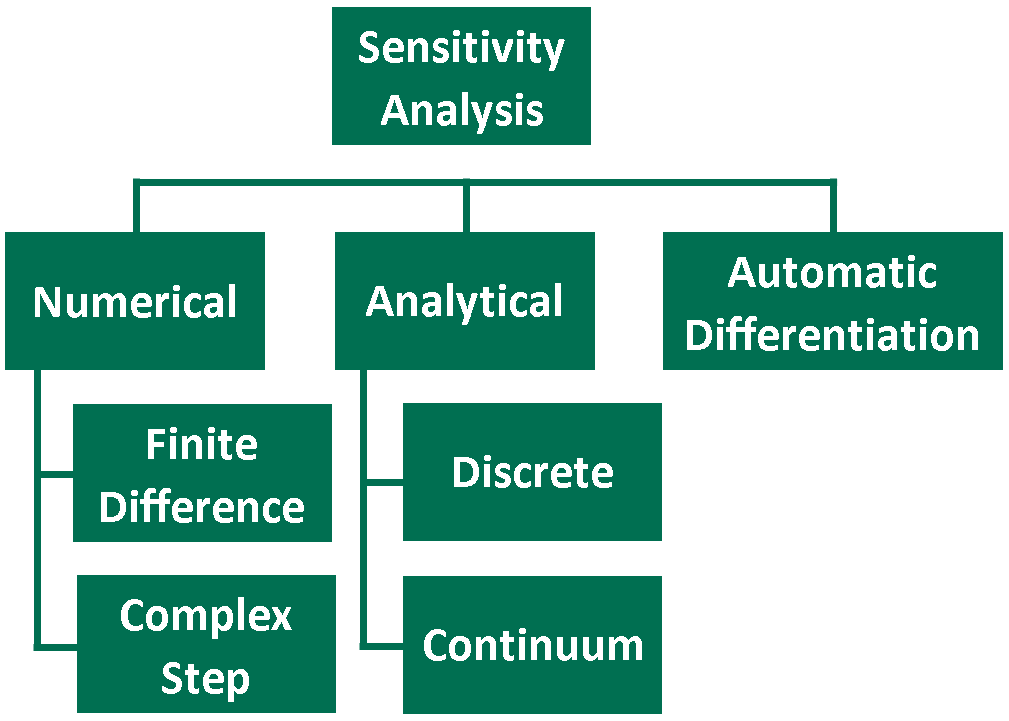
\includegraphics[height=7.00cm]{Chapter_1/figure/sensitivity_taxonomy.png}
	\caption{Sensitivity calculation techniques.}
	\label{fig:C1_sensitivityTaxonomy}
\end{figure}

The Finite Difference (FD) method is probably the easiest method to implement for calculating the sensitivity of a variable. The fact that they can be implemented even when a given computational model is a black box makes most gradient based optimzation algorithms perform finite differences by default when the used does not provide the required gradients. However, the computational cost associated with finite difference for large systems can become very large. For a system with $n$ number of design variables, the analysis needs to be done $n+1$ time to calculate the design sensitivities. Furthermore, to ensure the accuracy, convergence study needs to be done for selecting the appropriate step size for finite difference. The inaccuracy of finite differencing could result in convergence difficulties and inaccurate optimum results. On the other hand, Complex Step (CS) method avoids the loss of precision in finite differences approximation of sensitivities by employing complex arithmetic \cite{martins2003complex}. The complex step derivative is calculated as shown in Equation \eqref{eq:C1_compelxStepFormula}.

\begin{equation}\label{eq:C1_compelxStepFormula}
	\mathcal{F}^\prime\left(u; b\right) = \frac{\text{Im}\left[ \mathcal{F}\left(u; b + ih\right) \right]}{h}
\end{equation}

This means that we perturb the design variable by an imaginary value of $ih$ and then look at
the imaginary portion of the resulting response. Using the complex step method, we can choose a
small step size for $h$ without loosing accuracy. However, many commercial packages such as ANSYS or Nastran cannot handle complex arithmetic which makes the implementation of complex step method infeasible. Moreover, the high cost of finite difference is still associated with the complex method as well.

Automatic differentiation (AD) is based on the systematic application of the differentiation to computer programs \cite{naumann2012art}. In the AD approach, the chain rule of differentiation is applied to every line in the program. This assumes that the computer program consists of a sequence of explicit functions that act successively on some variables. Therefore, by differentiating each of these functions and applying the chain rule, it is possible to calculate the sensitivities. 

There has been many research on utilizing AD for optimization. Bischof et al. used AD for calculating the sensitivities using a CFD solver. They used ADIFOR for differentiating the source code of their CFD code (TLNS3D) which later used for calculating the sensitivity of a transonic flow to change in the boundary conditions. Hascout et al., also used AD for a sonic boom reduction under a supersonic aircraft. However, in all of these works, it is needed to have access to the source code and modify the solver extensively to calculate the sensitivities. This make the use of this method for general purpose codes infeasible since the source code is usually not available.

The short comings of numerical and AD techniques, fuels the research for more sophisticated methods for sensitivity calculation which are generally known as analytical methods. Formulation of the analytical sensitivities requires derivation of analytic sensitivity equations. These are obtained by differentiating the governing equations with respect to design variables such as shape of the boundaries. Analytical methods can be further categorized based on how the sensitivity equations derived and solved. Typically the continuum equations are solved using an approximate method which discretizes the governing equations. The Discrete Sensitivity Analysis (DSA) technique, differentiates the discretized governing equations with respect to design variables to get the analytical sensitivity equations \cite{choi2006structural}. This system of equations is later solved for analytical sensitivities.  

The discrete sensitivity analysis has been historically the method of choice to calculate the high-accurate sensitivity when the details of analysis are available \cite{arora1979methods}. This method has been adopted by the structural optimization community, and been applied to fluid-solid interaction problems as well. Reuther et al., used the discrete method for aerodynamic shape optimization of a complex aircraft configuration \cite{reuther1999constrained}. They used Euler flow as the aerodynamics theory where they optimized different configurations for transonic and supersonic regimes. However, they only focused on the flow. Martins et al., developed an adjoint method for sensitivity analysis for an aero-structural aircraft design framework where the sensitivities were computed using a coupled adjoint approach. The framework was used on a supersonic business jet to calculate the sensitivity of drag with respect to the shape (OML) of the aircraft. In their work, the discretization details of the solver needs to be known to calculate the sensitivities. As a matter of fact, source code modification is essential in all the other related research in the area as well \cite{gamboa2009optimization, pandya1997gradient, kim2001aerodynamic}.

As mentioned before, sensitivity calculation is the essential part of gradient based optimization. However, many general purpose solvers do not have this capability. This is even more prominent in the fluid mechanics community where none of the available commercial software packages such as ANASYS Fluent or CFX has analytical sensitivity analysis capabilities. In optimization loop, they relay on finite difference as a method for sensitivity calculation. As mentioned in the previous paragraph, for the discrete sensitivity methods, intimate knowledge and access to the source codes of these software is needed to calculate the sensitivities. However, the source code is usually inaccessible and very complex. Therefore, there is a great interest in sensitivity calculation techniques which require minimum knowledge of the analysis code. This can be achieved using the sensitivity formulation that operate on the governing equations before they are discretized. These method are commonly known as Continuum Sensitivity Methods \cite{haftka1989recent}.

The Continuum Sensitivity Analysis (CSA), involves solving a set of partial differential equations named the continuum sensitivity equations (CSEs) to get the analytical sensitivities. When deriving the CSEs, the governing equations can either be differentiated in local or total form. The difference between local and total differentiation depends on the Lagrangian or Eulerian representation of the governing equations. In the general case of continuum mechanics,  displacement and velocity are vector valued functions. I any application, we have the choice of writing these vectors as functions of the position of material particles before deformation. This is called the Lagrangian description of motion and is really helpful for visualizing the deformations. This technique is mostly adopted in solid mechanics where we track the material points as the deformations are usually assumed to be small. However, in the fluid flow problems, since it is generally hard to identify a reference configuration and the deformations are large, it is preferable to write the displacement and velocities as functions of the deformed position of the particles. These quantities are now defined for a particular point in space that does not move with the particles. This is called the Eulerian description of motion.  As CSA was matured over the year, the computational fluids community adopted the local CSEs, since its formulation is consistent with the governing equations \cite{borggaard1997pde, hristova2006continuous}. The structural optimization community adopted the total formulation for the sensitivities since its formulation was consistent with the Lagrangian formulation of structural mechanics. Nevertheless, the total and local formulations for the sensitivities can be converted to each other. This will be explained in more details in next chapter.

Overally, the sensitivity analysis in general is more matured is the concept of structural optimization than for problems of fluid dynamics. Nevertheless, neither of these disciplines do not typically employ CSA for the sensitivity calculation. Aurora and Haug \cite{Arora}, followed by Dems and Mroz \cite{Dems-Mroz}, were among the first to develop the concept of CSA for structural optimization. They modeled the sensitivities as functionals therefore they were able to convert the sensitivity integrals over the entire domain to the integrals over the boundaries. Although using the approach it is possible to reduce the cost of the simulation, accurate values of functionals are required at the boundaries. This is not always achievable especially for finite element analysis where the solution accuracy drops near the boundaries. The lack of applicability of CSA in structural optimization is due to the complicated definition of the boundary conditions and maturity of discrete methods for the sensitivity calculation. 

The first application of CSA in optimization problems for fluid dynamics is the work by Borggaard and Burns \cite{borggaard1995sensitivity} for shape sensitivity analysis of inviscid supersonic flows over rigid bodies. Stanley and Stewart \cite{stanley2002design} applied CSA in a fluid mechanics discipline with a goal for aerodynamic design. Pelletier and Etienne have applied CSA to numerous fluid-structure interaction (FSI) problems \cite{etienne2005general} focused mainly on sensitivities of fluid flow parameters near the structure. Liu and Canfield have employed CSA for shape optimization of nonlinear structures subject to an aeroelastic gust response \cite{liu2013equivalence}. They used the finite element method to solve the potential flow around an airfoil and applied CSA to find the airfoil pressure coefficient sensitivity with respect to the maximum camber. 

In almost all of the research done on sensitivity calculation of flow field to shape design variable, body conformal grids were used. The conforming mesh methods consider the interface conditions as physical boundary conditions, which treat the interface location as part of the solution and requires meshes that conform to the interface. Using this approach it is possible to represent the solid boundary shape with good accuracy. However, due to the coupling of fluid mesh topology and solid boundary shape, with the movement and/or deformation of the solid structure, re-meshing (or mesh-updating) is needed. Although conforming mesh methods have been widely used in many FSI problems, they are cumbersome, if not impossible, to apply to problems with large deformations \cite{sahin2009arbitrary}. The other shortcoming of body-conformal grids, is the effect of mesh deformation on the sensitivity analysis. Since the computational domain is affected by change in the shape of the boundaries, it is required to calculate the mesh sensitivities as well \cite{liu2013boundary}. This adds to the computational cost of calculating  sensitivities.

The shortcoming of a robust grid generation and the additional cost of calculating mesh sensitivities motivated an important research effort to develop a method that does not require fluid domain mesh modification for the optimization iterations. On of the possible candidates to achieve this goal, is the use of Immersed Boundary (IB) methods to decouple the fluid mesh from the shape of solid domain.
% ---------------------------------------------------------------------------------------------
\subsection{Immersed Boundary Method}
Traditionally the simulation methods for flow over complex bodies are based on a body-fitted multi-block or unstructured grid methods. However, in the last decade another class of techniques, called immersed boundary methods, have been introduced to model the flow around solid boundaries. The term immersed boundary is first used by Peskin \cite{peskin1977numerical} to simulate the blood flow through heart valves. What distinguishes this method from the other methods of representing the solid boundaries is that the flow is solved on the Cartesian grid that does not conform to the solid boundaries. Therefore, the mesh generation is greatly simplified and in case of moving/deforming boundaries, there is no need to update the mesh during the simulation. A separate formulation is used to impose the effect of the boundaries on the solution of the equations.

Consider the simulation of flow past a circular cylinder as shown in Figure \ref{fig:C1_conformalVSnonconformal}. Generating structured or unstructured grids is achieved in two steps. First, a surface grid covering the boundaries is generated. This is then used as a boundary condition to generate a grid in the volume occupied by the fluid. The differential form of the governing equations is then transformed to a curvilinear coordinate system aligned with the grid lines \cite{anderson1995computational}. If a finite-volume technique is employed, then the integral form of the governing equations is discretized and the geometrical information regarding the grid is incorporated directly into the discretization. If an unstructured grid is employed, then either a finite-volume or a finite-element methodology can be used.

%
\begin{figure}[h]
	\centering
	\subfigure[Conforming mesh, $t = t_1$]
	{
	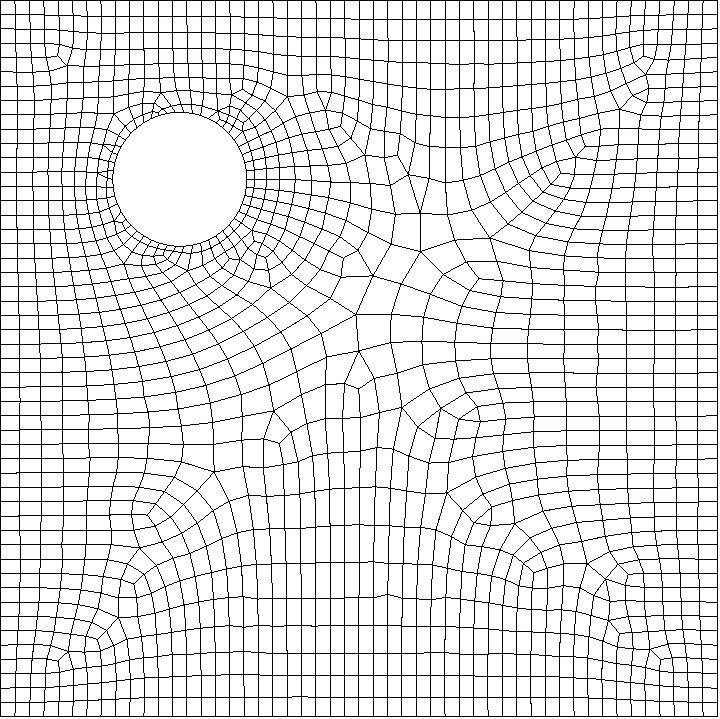
\includegraphics[height=5.0cm]{Chapter_1/figure/conforming_t1.jpg}
	}
	\quad
	\subfigure[Conforming mesh, $t = t_2$]
	{
	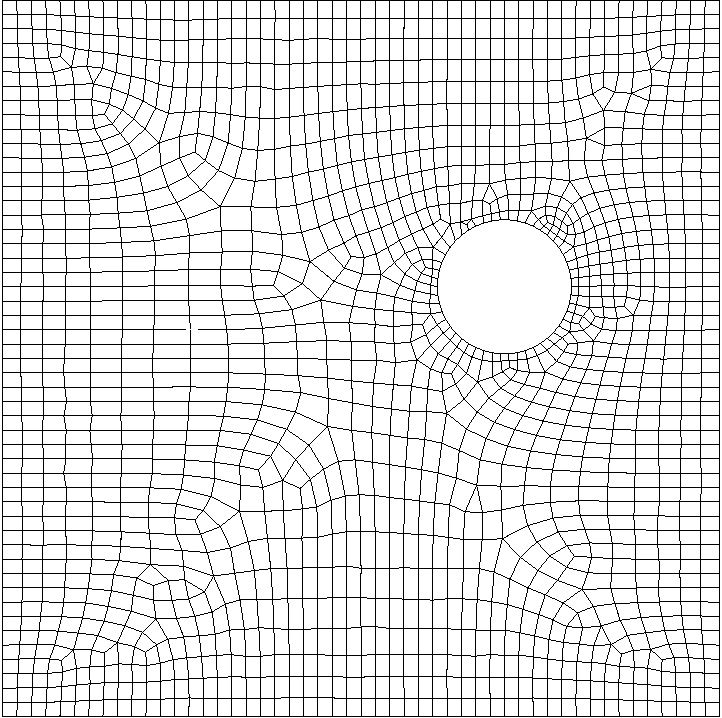
\includegraphics[height=5.0cm]{Chapter_1/figure/conforming_t2.jpg}
	}
	\\
	\subfigure[Nonconforming mesh, $t = t_1$]
	{
	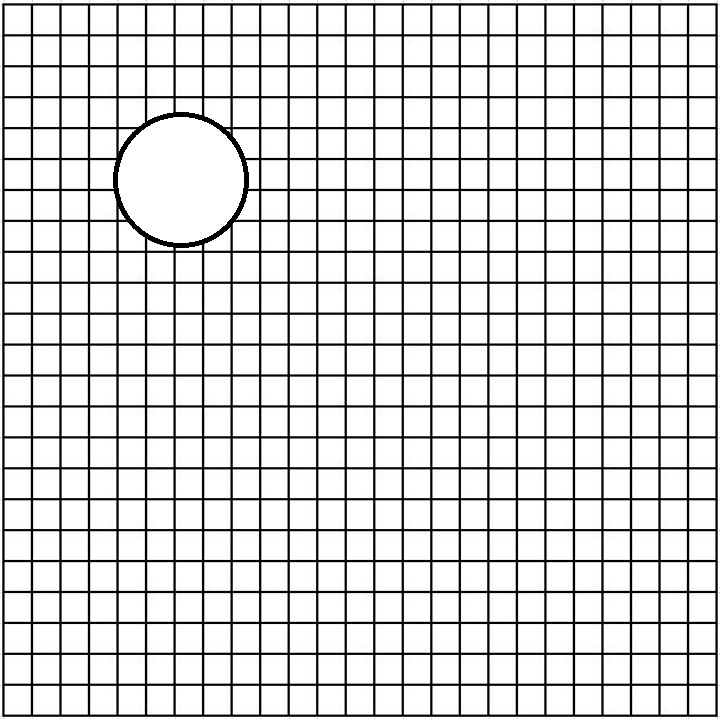
\includegraphics[height=5.0cm]{Chapter_1/figure/nonconforming_t1.jpg}
	}
	\quad
	\subfigure[Nonconforming mesh, $t = t_2$]
	{
	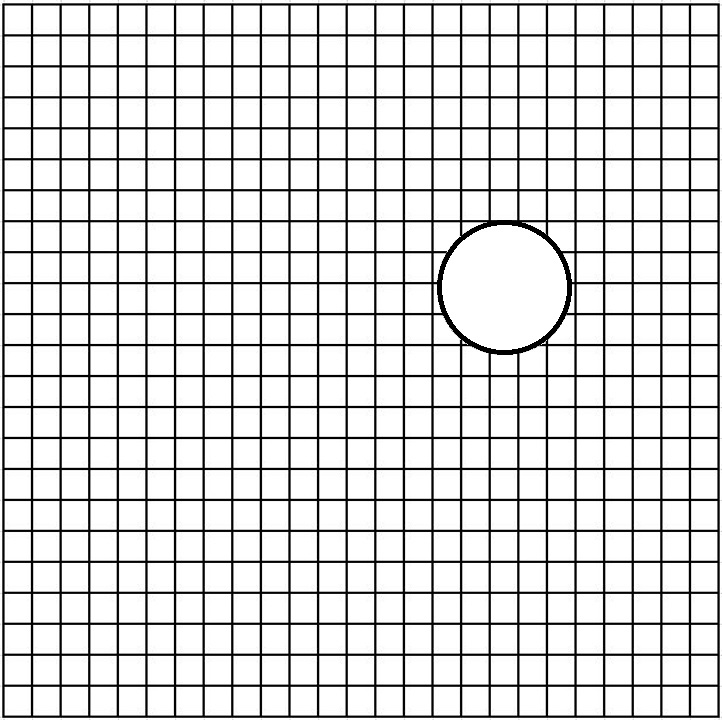
\includegraphics[height=5.0cm]{Chapter_1/figure/nonconforming_t2.jpg}
	}
	\caption{Example of conforming and nonconforming meshes.}
	\label{fig:C1_conformalVSnonconformal}
\end{figure}
%

Non-body conformal Cartesian grid can also be utilized for this simulation as shown in Figure \ref{fig:C1_conformalVSnonconformal}. In this approach the IB would still be represented through some means such as a surface grid, but the Cartesian volume grid would be generated with no regard to this surface grid. Thus, the solid boundary would cut through this Cartesian volume grid. Because the grid does not conform to the solid boundary, incorporating the boundary conditions would require modifying the equations in the vicinity of the boundary. Assuming that such a procedure is available, the governing equations would then be discretized using a finite-difference, finite-volume, or a finite-element technique without resorting to coordinate transformation or complex discretization operators.

Depending on how the effect of solid boundaries are imposed, IB methods can be divided into four categories: i) Continuous forcing, ii) discrete forcing, iii) penalization, and iv) cut-cell method.

\subsubsection{Continuous forcing method}
This is the originaly used by Peskin \cite{peskin1977numerical} and later developed by others researchers \cite{saiki1996numerical, zhu2003interaction, beyer1992analysis}. In this approach, the boundary configuration is described by a curve $x(s,t)$ (Lagrangian nodes) where the location of each point on this boundary is governed by its equations of motion. The forces that the curve $x(s,t)$ exerts on the fluid is calculated buy the constitutive law of the curve $x(s,t)$ that relates the displacements to stress values. These stress values are transferred to the Navier-Stokes (NS) (Eulerian nodes) for the fluid by means of a Dirac delta function. Practical implimentation of this method resets in representing the Dirac delta function as a discrete function that has the same properties. This method is applied to variety of problems, including Cardiac blood flow \cite{peskin1989three}, animal locomotion \cite{fauci1988computational}, multiphase flows \cite{kempe2015imposing}, and particle sedimentation \cite{uhlmann2005immersed}.

Peskin's method is well suited for the elstic boundaries. For stiff boundaries, the constitutive laws of the solid boundaries will result in instabilities in the solution of governing equations \cite{mittal2005immersed}. The virtual boundary method of Goldstein \cite{goldstein1993modeling} enables us to handle these rigid boundaries. The main idea of this approach is the same as Peskin's method where the solid boundary is treated as a virtually existing surface embedded in the fluid. The force on this surface is calculated by the requirement that the fluid velocity should satisfy the no-slip condition. Since this body force is not known a priori, it is calculated in a feedback way.

\subsubsection{Discrete forcing method}
This discrete formulation of IB method was first introduced by Mohd-Yusof \cite{mohd1997combined} for addressing the time penalties associated with the simulation involving moving boundaries. The main idea of this technique is same as the virtual boundary method where a force term is added to the momentum equations to represent the solid boundary. However, in the current approach the momentum equation manipulation is done in the discrete manner. In the work of Mohd-Yusof \cite{mohd1997combined} and Verzicco et al. \cite{verzicco1998complex} this is done by modifying the discretization stencil in the vicinity of the boundary curve so that the velocity values on this boundary satisfies a pre-defined condition. The major advantage of this approach is the lack of user specified parameters however, its implementation depends strongly on the discretization approach used for the analysis. Therefore, it cannot easily implemented in commercial codes. This implementation of discrete forcing method has be applied to many different problems such as turbulent flow inside an internal combustion engine \cite{verzicco1998complex}, flow past 3D bluff bodies \cite{verzicco2002large}, and cylindrical stirred tank \cite{iaccarino2003immersed}.

\subsubsection{Penalization method}
The penalization method is based on the Brinkman equation that describes the flow of a fluid through a porous medium. The Brinkman equation is analogous to Fourier's laws in heat conduction and Ohm's law in the field of electrical engineering \cite{durlofsky1987analysis}. This approach was first proposed by Arquis and Caltagirone where they imposed the boundary conditions by adding the penalization terms to the momentum equations \cite{arquis1984conditions}. The main idea of this approach is to model the solid obstacles as a porous medium with the porosity of $\mathcal{K}$. The porosity is a measure of the void spaces in a material. Therefore, by selecting low values for porosity, the porous domain acts as a solid wall. It has be argued that the solution of the penalized incompressible NS equations converges to the exact solution as the porosity approaches zero \cite{angot1999analysis} however in the practical implementation, extreme low values for porosity will result in systems with a very large stiffness and numerically unstable. To apply the porosity within the solid domain, a Heaviside function is used by different researchers \cite{gazzola2011simulations, kevlahan2001computation}.

\subsubsection{Cut-cell method}
In the cut-cell methods, the grid cells are cut by the solid boundary and reshaped so that they form a boundary-conforming, unstructured gird. This is shown in Figure \ref{fig:C1_cutCellMesh}.

\begin{figure}[h]
	\centering
	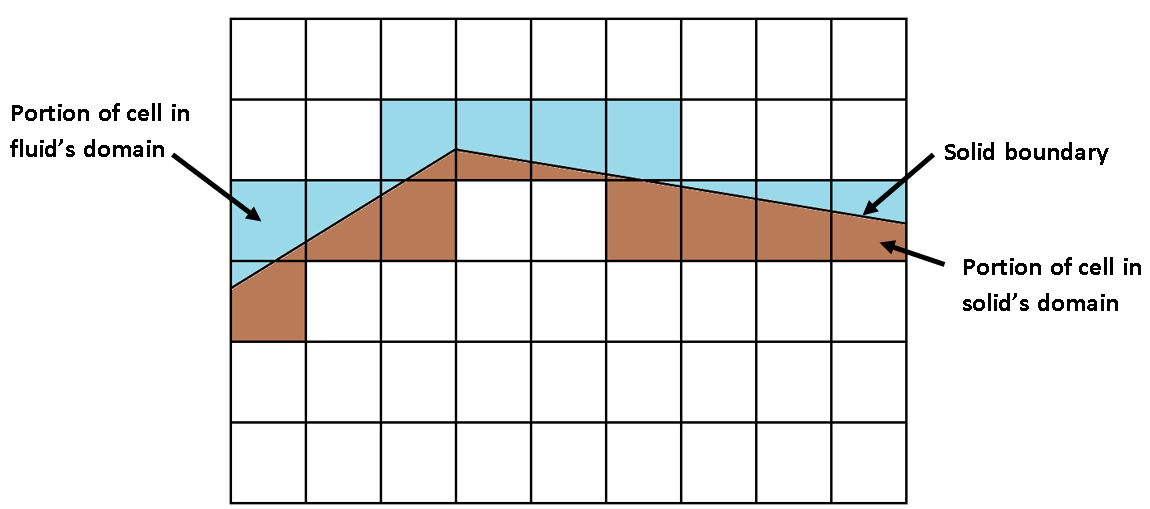
\includegraphics[height=7.0cm]{Chapter_1/figure/cut_cell_mesh}
	\caption{Modified mesh near the solid boundary for cut cell method.}
	\label{fig:C1_cutCellMesh}
\end{figure}

The cut-cell method was first introduced Clarke \cite{clarke1986euler} for inviscid flows. This method have been applied to both collocated and staggered grids \cite{kirkpatrick2003representation} however, most of the applications were focused on 2D flows \cite{hu2006conservative, udaykumar1999computation}. This is because of the many possibilities for the geometrical shape of the cut-cell, that makes the flux calculation and therefore numerical implementation extremely difficult.

% ---------------------------------------------------------------------------------------------
\subsection{Sensitivity analysis for IB method}
The body of the research done in the immersed boundary community has been concentrated on the improvement of the method and resolving the stability issues. However, there has not been much effort in the sensitivity calculation of a IB formulation. Most of the sensitivity analysis research is developed for the penalization framework. Borrvall and Petersson applied the penalization method for topology optimization of fluids in Stokes flow \cite{borrvall2003topology}. They used the discrete sensitivity analysis to calculate the sensitivity of fluid pressure to the shape of the boundaries. They used this technique to optimize the shape of a diffuser and also a pipe bend. They verified their methodology for outflow problems as well, where they optimized the shape of solid domain to maintain the least possible pressure drop. They also had constraint on the volume of domain that can be penalized.  Challis and Guest investigated the level set formulation for the topology optimization of fluids in Stokes flow \cite{challis2009level}. They used the penalization technique to formulate their problem where they were able to accurately model the no-slip condition on the solid boundaries. They implemented the Topological sensitivities in their solver where they used power dissipation minimization to optimize the shape of a diffuser and a connecting pipe in 3D.

The penalization method is probably the easiest of the IB methods to implement. This is because it does not have a free parameter such a virtual boundary method and does not depend on the discretization such as discrete sensitivity methods. Moreover, no interpolation is needed for applying penalization method to a computational domain. The nodes are assigned porosity based on the relative location to the